%% Sets aspect ratio to 16:10, and frame size to 160mm by 100mm
% Please, do not use old-school 4:3 ratio anymore:)
\documentclass[aspectratio=1610]{beamer}
% všechny soubory jsou v utf-8
\usepackage{ucs}% pro kódování UTF-8
\PrerenderUnicode{ěščřžýáíéĚŠČŘŽÝÁÍÉďťňĎŤŇůúÚóÓ} % předkreslení diakritiky, možno přidat/ubrat znaky podle potřeby	

%% Select your favorite language
%\usepackage[english]{babel} % Multilingual support for LaTeX
\usepackage[czech]{babel}
\usepackage[IL2]{fontenc}% csr fonty (pokud jsou nainstalovány česká postscriptová mísma)

\usepackage[utf8]{inputenc} % Accept different input encodings
\usepackage{graphicx} % Enhanced support for graphics
\usepackage{listings} % Typeset source code listings using LaTeX
\usepackage{color} % Colour control for LaTeX documents
\usepackage{bm} % Colour control for LaTeX documents

\usepackage{makecell}
\usepackage{multirow}

\renewcommand\theadalign{cc}
\renewcommand\theadfont{\bfseries}
\renewcommand\theadgape{\Gape[4pt]}
\renewcommand\cellgape{\Gape[4pt]}

\usepackage{setspace}

%% Copy your favorite logo from "vut_logo_archive/" to root folder 
% and rename file to "logo.png"

%% Select color theme
\usepackage[FSI]{themevut}

\usepackage{parskip}
\usepackage{media9}	

\lstset{frame=tb,
	language=C++,
	aboveskip=3mm,
	belowskip=3mm,
	showstringspaces=false,
	columns=flexible,
	basicstyle={\small\ttfamily},
	numbers=none,
	numberstyle=\tiny,
	breakatwhitespace=true,
	tabsize=3,
	breaklines=true
}
% ----------------------------------------------------------------------
% TITLE PAGE
% ----------------------------------------------------------------------

% The short title appears at the bottom of every slide, the full title
% is only on the title page.
\title[Sémantická segmentace obrazu pomocí CNN]
{Sémantická segmentace obrazu pomocí konvolučních neuronových sítí}

% Type of project, i.e. Bachelor, Master, PhD, etc.
\subtitle
{Diplomová práce}

% Your name
\author[Bc. Filip Špila]
{Bc. Filip Špila \\
	\texttt{filipspila@gmail.com}}

% Your institution
\institute
{Ústav mechaniky těles, mechatroniky a biomechaniky \\
	Vysoké učení technické v Brně
}

% Date, can be changed to a custom date
\date{\today}

% Logo on title page
\titlegraphic{
\includegraphics[height=.1\textheight]{logo4.png}}

\begin{document}
	
	% ----------------------------------------------------------------------
	% PRESENTATION SLIDES
	% ----------------------------------------------------------------------
	
	\begin{frame}
	% Print the title page as the first slide
	\titlepage
	\end{frame}
% ----------------------------------------------------------------------

\begin{frame}{Sémantická segmentace}
	\textbf{Cíle sémantické segmentace}
	\begin{itemize}
	\item Přiřadit každému pixelu v obrázku právě jednu třídu objektu (auto, člověk, zvíře, ...)
	% Narozdil od klasifikace obrazu jako celku
	\item Provádět segmentaci co nejpřesněji
	% Tedy s presnym vykreslenim hranice kazdeho objektu
	\item Zajistit, aby algoritmus uměl generalizovat
	% Tedy aby spravne klasifikoval objekty bez ohledu na svetelne podminky, ruzne nedokonalosti atp.	
	\end{itemize}
	\vspace{5mm}		
	\begin{center}	
		\includemedia[
		width=0.4\linewidth,
		height=0.2\linewidth,
		addresource=cut.mp4,
		activate=pagevisible,
		passcontext, 
		playbutton=none,
		flashvars={				
			source=cut.mp4
			&autoPlay=true
			&loop=false
		}
		]{}{VPlayer.swf}	
	\end{center}
\end{frame}
% ----------------------------------------------------------------------
% https://cs.overleaf.com/learn/latex/Lists

\begin{frame}{Cíle práce}
\begin{enumerate}
	\item Nastudování problematiky segmentace obrazu pomocí konvolučních neuronových sítí
	\item Výběr perspektivní architektury sítě spolu s její implementací
	\item Vytvoření vlastní trénovací množiny obrázků
	\item Vytvoření segmentovaného obrazu
	\item Vyhodnocení úspěšnosti segmentace
\end{enumerate}	
\end{frame}

% ----------------------------------------------------------------------
% https://en.wikibooks.org/wiki/LaTeX/Floats,_Figures_and_Captions
\begin{frame}{Neuronové sítě a učení s učitelem}
\textbf{Proč pro segmentaci místo klasických metod použít neuronovou síť?}
\begin{itemize}
	\item Dovede velmi dobře aproximovat silně nelineární funkce
	\item Potřebuje jen mírně předzpracovaná data
	\item Detekuje obecné vzory v datech = dovede lépe generalizovat
	\item Algoritmus je robustnější
	
\end{itemize}
\end{frame}
% ----------------------------------------------------------------------
% https://en.wikibooks.org/wiki/LaTeX/Floats,_Figures_and_Captions
\begin{frame}{Neuronové sítě a učení s učitelem}
\textbf{Úloha neuronové sítě}
\begin{itemize}
\item Aproximace obecné funkce $y=f(x;\phi)$ funkcí $ y^* = f^*(x;\phi)	$ řešením:
\vspace{3mm}					
\begin{gather}
\phi \leftarrow \, \text{arg min} \, L(y, f^*(x;\phi))	
\end{gather} 

Funkce $ L $ se nazývá \textbf{hodnotící funkce} (míra spokojenosti s výstupem). Parametry $ \phi $ jsou nalezeny trénováním sítě neboli optimalizací \textit{L}
\item Jakmile trénování skončí, nastává \textbf{inference} = používání sítě s již pevnými parametry $ \phi $ a novými daty
\end{itemize}
\end{frame}
% ----------------------------------------------------------------------
\begin{frame}{Trénování neuronové sítě}
\textbf{Gradientní optimalizace hodnotící funkce - kroky}
\begin{enumerate}
	\item Derivace hodnotící $ L $ funkce podle daného parametru $ \phi $: $ \frac{\partial L}{\partial \phi} $
	\item Změna parametru \textbf{proti} směru derivace (hledání minima)
	\begin{gather}
	\delta \phi = - \eta \frac{\partial L}{\partial \phi}
	\end{gather}	
	\noindent kde $ \eta $ je rychlost učení. Další detaily záleží na konkrétním algoritmu.	
\end{enumerate}
	\begin{center}		
	\includemedia[
	width=0.35\linewidth,
	height=0.25\linewidth,
	addresource=opti.mp4,
	activate=pagevisible,
	passcontext, 
	playbutton=none,
	flashvars={				
		source=opti.mp4
		&autoPlay=true
		&loop=true
	}
	]{}{VPlayer.swf}			
\end{center}
\end{frame}
% ----------------------------------------------------------------------
\begin{frame}{}
\centering
{\Large Konvoluční neuronové sítě (CNN)}	
\end{frame}
% ----------------------------------------------------------------------
\begin{frame}{CNN - konvoluční neuronové sítě}
	\begin{figure}[h]
	\begin{center}
		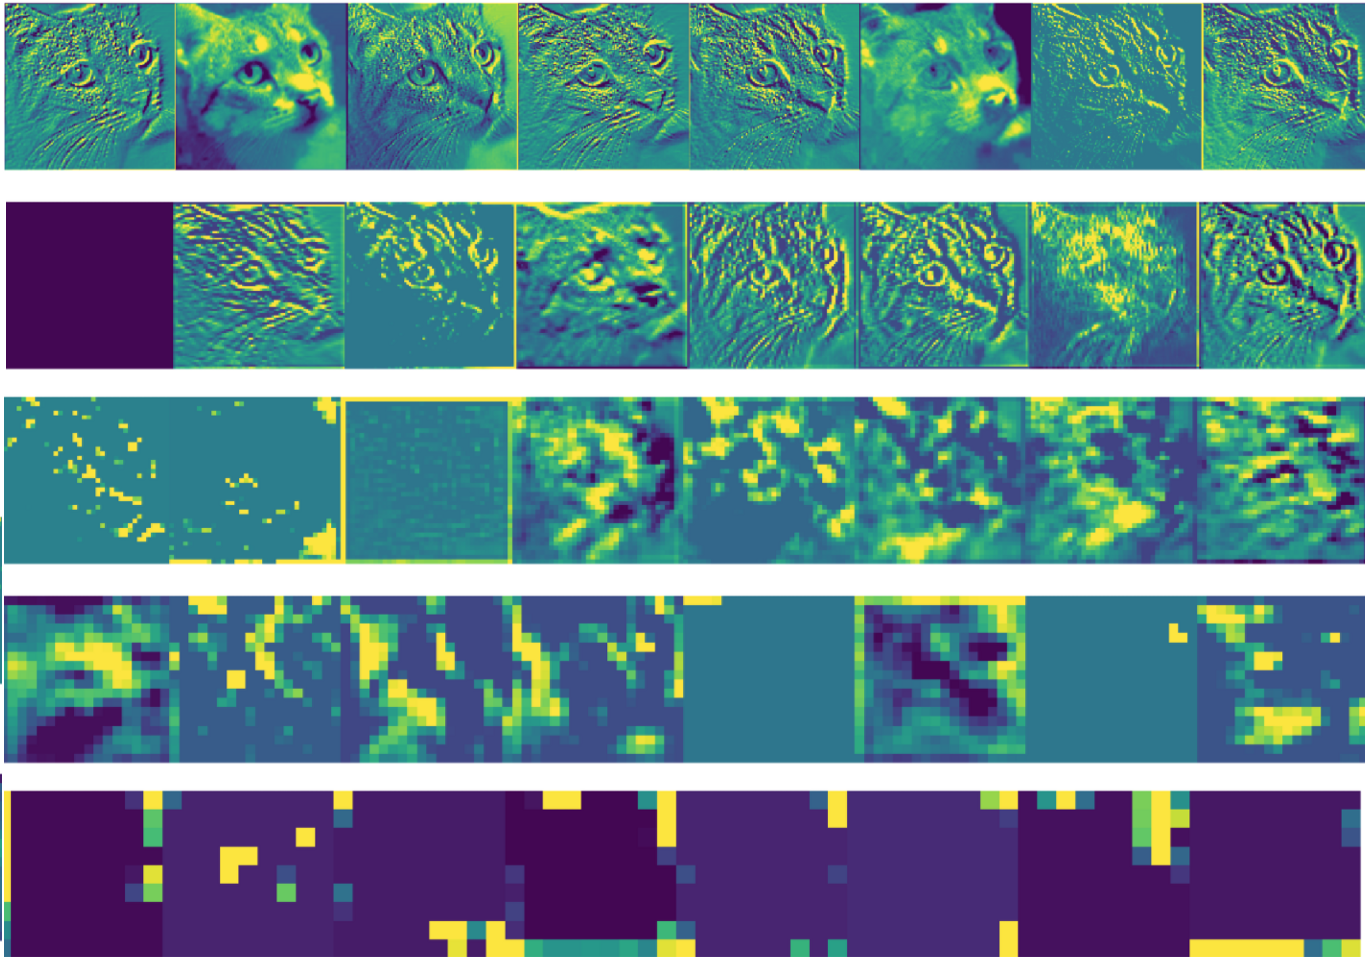
\includegraphics[width=9cm, keepaspectratio]{maps.png}
	\end{center}
	\caption{Mapy prvků v obraze} 	
\end{figure}
\end{frame}
% ----------------------------------------------------------------------
\begin{frame}{Segmentace - architektura enkodér-dekodér}
\begin{figure}[h]
	\begin{center}
		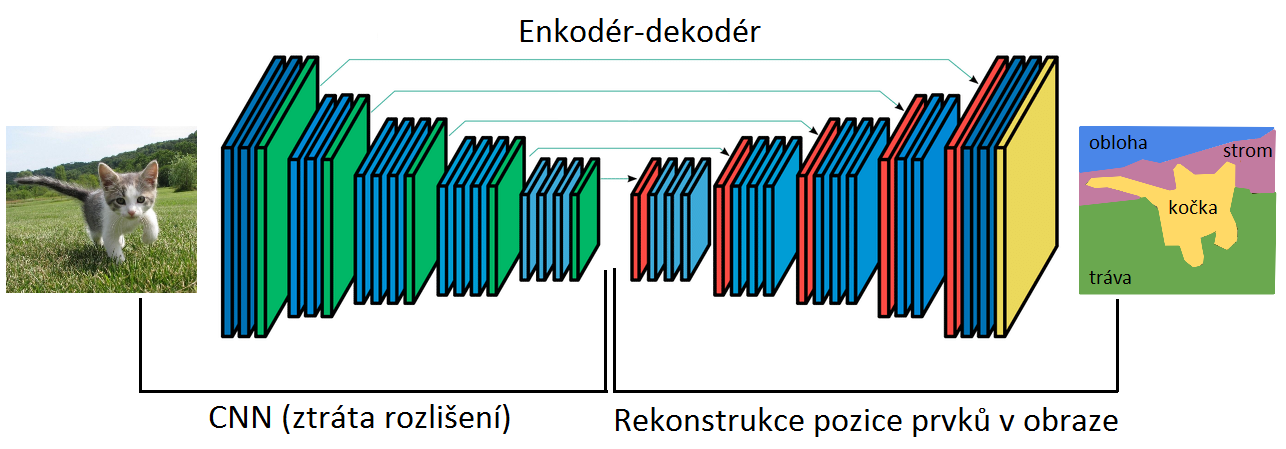
\includegraphics[width=15cm, keepaspectratio]{segnet.png}
	\end{center}
	\caption{Architektura enkodér-dekodér} 	
\end{figure}
\end{frame}
% ----------------------------------------------------------------------
\begin{frame}{Trénování architektur 'enkodér-dekodér'}
\textbf{Hlavní trénovatelné parametry}

\begin{itemize}
	\item Hodnoty konvolučních jader (jednotlivých filtrů)
	% vahy vazeneho prumeru
	\vspace{5mm}		
	\begin{center}		
	\includemedia[
	width=0.4\linewidth,
	height=0.3\linewidth,
	addresource=convo.mp4,
	activate=pagevisible,
	passcontext, 
	playbutton=none,
	flashvars={				
		source=convo.mp4
		&autoPlay=true
		&loop=true
	}
	]{}{VPlayer.swf}			
	\end{center}	
\end{itemize}

\end{frame}
% ----------------------------------------------------------------------
\begin{frame}{}
\centering
{\Large Praktická část práce}	
\end{frame}
% ----------------------------------------------------------------------
\begin{frame}{SegNet}
\textbf{SegNet = segmentační CNN typu enkodér-dekodér}
\begin{itemize}
	\item Vytvořeno na univerzitě v Cambridge
	\item Originální implementace dostupná online	
	\item Existuje i zjednodušená verze (méně vrstev sítě)
\end{itemize}
\begin{figure}[h]
	\begin{center}
		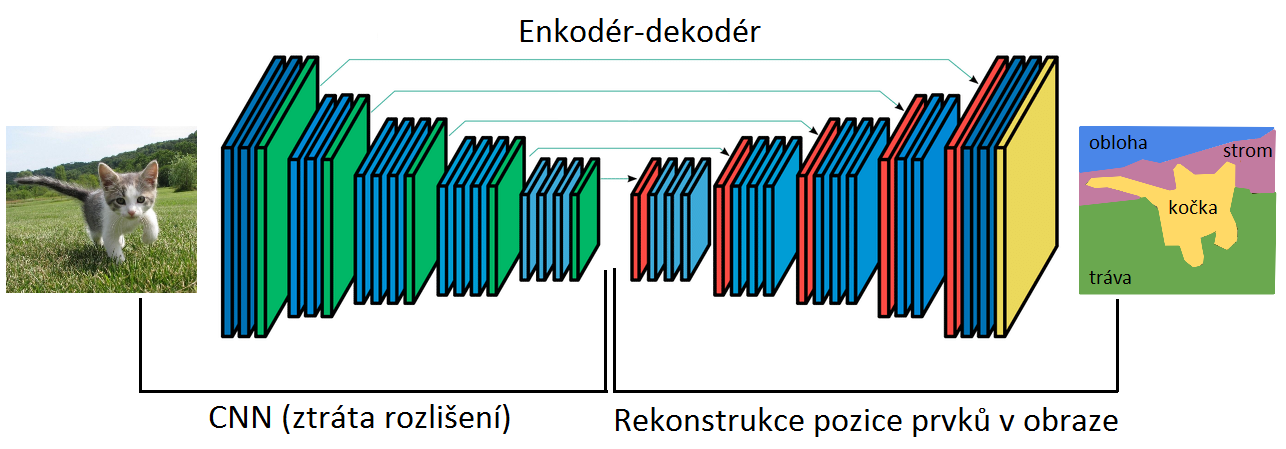
\includegraphics[width=10cm, keepaspectratio]{segnet.png}
	\end{center}
	\caption{SegNet} 	
\end{figure}
\end{frame}
% ----------------------------------------------------------------------
\begin{frame}{Bayesian SegNet}
\textbf{Bayesian SegNet}
\begin{itemize}
	\item Architektura téměř shodná se SegNetem 
	\item Navíc dovede určit nejistotu segmentace
	\item Parametry sítě se náhodně nulují = 'více architektur najednou'
\end{itemize}
\vspace{5mm}
\begin{figure}[h]
	\begin{center}
		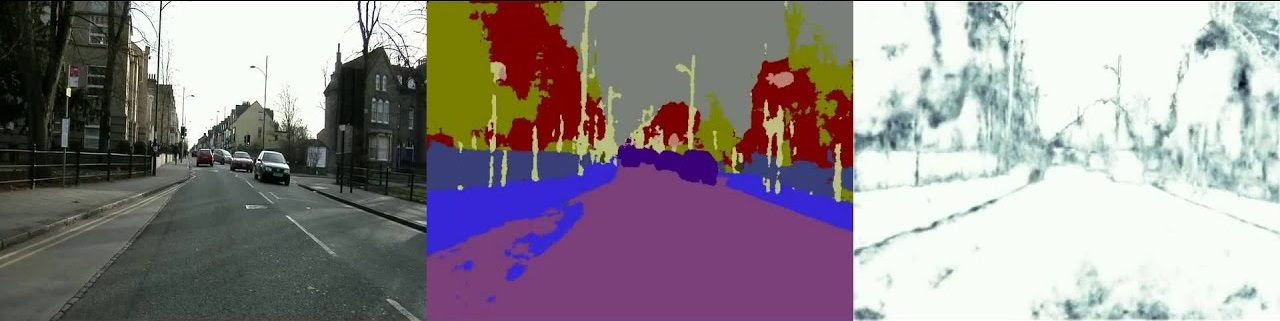
\includegraphics[width=10cm, keepaspectratio]{bayesian.jpg}
	\end{center}
	\caption{Bayesian SegNet} 	
\end{figure}
\end{frame}
% ----------------------------------------------------------------------
% https://tex.stackexchange.com/questions/130109/cant-insert-code-in-my-beamer-slide
\begin{frame}[fragile]{Implementace variant SegNetu v Caffe}
	\begin{columns}
		\column{0.6\textwidth}	
		{\setstretch{1.25}
			\begin{itemize}	
				\item Caffe je knihovna pro neuronové sítě		
				\item Abstrakce vrstev CNN - snadné vytvoření architektury
				\item Nutné sestavit ze zdrojového kódu, nejlépe pod Linuxem		
			\end{itemize}
		}
		\vspace{5mm}
		\begin{figure}[h]
			\begin{center}
				
\includegraphics[width=4cm, keepaspectratio]{caffe-logo.png}
			\end{center}	
			\caption{Caffe logo} 	
		\end{figure}
	
		\column{0.3\textwidth}		
\begin{lstlisting}
	layer {
	bottom: "conv1"
	top: "conv1D"
	name: "conv1D"
	type: "Conv"
	param {
	lr_mult: 1
	decay_mult: 1
	}
	param {
	lr_mult: 2
	decay_mult: 0
	}			
	\end{lstlisting}		
	\end{columns}
\end{frame}
% ----------------------------------------------------------------------
\begin{frame}{Nastavení prostředí pro Caffe}
	\begin{columns}[T]
	\column{0.6\textwidth}
    {\setstretch{1.5} 		
		\textbf{Hlavní přípravné kroky}
		\begin{enumerate}
			\item Volba hardwaru pro trénování - grafická karta, SSD
			\item Nastavení Linuxu (Ubuntu) pro kompilaci Caffe
			\begin{itemize}
				\item Knihovna CUDA pro paralelizaci výpočtů
				\item Všechny potřebné balíky ve správné verzi
			\end{itemize}
			\item Kompilace a testování Caffe					
		\end{enumerate}
	}
	\column{0.3\textwidth}
	\begin{figure}[h]
		\centering
			
\includegraphics[width=4cm, keepaspectratio]{ubuntu.jpg}			
	\end{figure}
	\end{columns}
\end{frame}
% ----------------------------------------------------------------------
\begin{frame}{Trénování SegNetu + Bayesian SegNetu}
\textbf{Vybraná úloha pro segmentaci}
	\begin{itemize}
		\item Rozpoznávání cesty na snímcích z městského parku
		\item Nutné vytvořit vlastní trénovací dataset (celkem 2600 snímků)
	\end{itemize}
	\vspace{5mm}
	\begin{figure}[h]
	\centering
	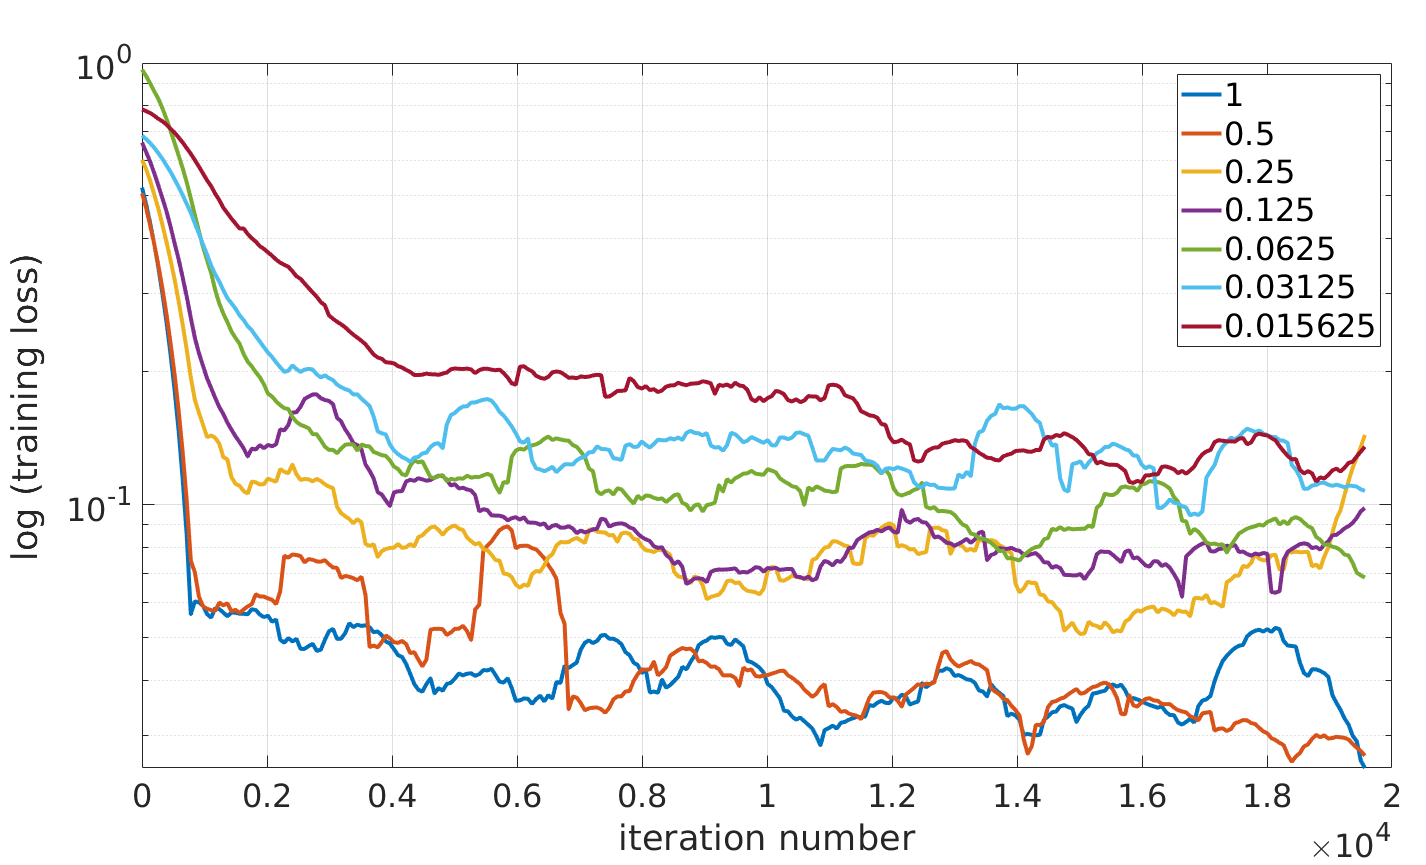
\includegraphics[width=13cm, keepaspectratio]{result.png}			
	\end{figure}	
\end{frame}
% ----------------------------------------------------------------------
\begin{frame}{Trénování SegNetu + Bayesian SegNetu}
\textbf{Data pro trénování}
\begin{itemize}
	\item V případě segmentace množina dvojic obrázků: \textbf{scéna + segmentační maska}
	\item Cílem je zabránit přeučení sítě
	\begin{itemize}
		\item (trénovací + validační) + testovací data
	\end{itemize}
	\item Čím více, tím lépe (co největší definiční obor aprox. funkce)
\end{itemize}
\begin{figure}[h]
	\begin{center}
		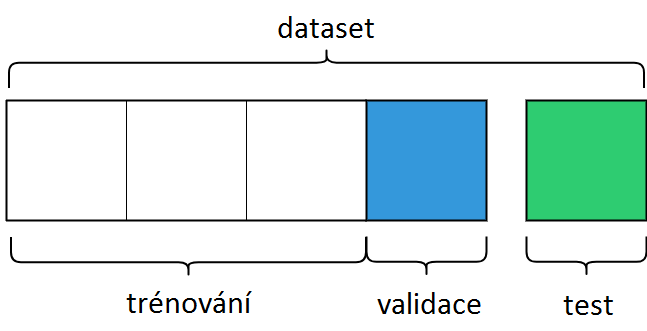
\includegraphics[width=6cm, keepaspectratio]{dataset.png}
	\end{center}
	\caption{Rozdělení datové množiny} 	
\end{figure}

\end{frame}
% ----------------------------------------------------------------------
\begin{frame}{Trénování SegNetu + Bayesian SegNetu}
\textbf{Přenastavení implementace variant SegNetu}
	\begin{itemize}
		\item Změna počtu tříd klasifikace (pro třídy \textbf{'pozadí'} + \textbf{'cesta'})
		\item Experimentální volba parametrů (rychlost učení, optimalizační algoritmus)
		\item Stejné pro SegNet + Bayesian SegNet
	\end{itemize}
\end{frame}
% ----------------------------------------------------------------------
\begin{frame}{Výsledky trénování}
\begin{center}
	\includemedia[
	width=0.9\linewidth,
	height=0.4\linewidth,
	addresource=project2.mp4,
	activate=pagevisible,
	passcontext, 
	playbutton=none,
	flashvars={				
		source=project2.mp4
		&autoPlay=true
		&loop=true
	}
	]{}{VPlayer.swf}
\end{center}
\end{frame}
% ----------------------------------------------------------------------
\begin{frame}{Výsledky trénování}
\centering
\includemedia[
width=0.55\linewidth,
height=0.5599\linewidth,
addresource=project1.mp4,
activate=pagevisible,
passcontext, 
playbutton=none,
flashvars={				
	source=project1.mp4
	&autoPlay=true
	&loop=true
}
]{}{VPlayer.swf}
\end{frame}
% ----------------------------------------------------------------------
% https://en.wikibooks.org/wiki/LaTeX/Tables
\begin{frame}{Výsledky trénování v číslech}
\renewcommand{\arraystretch}{1.5}
%\newcolumntype{C}{>{\centering\arraybackslash}p{3em}}
\begin{table}[h]
	\centering	
	\begin{tabular}{|c|c|c|c|c|}
		\hline
		\thead{Architektura} & \thead{Úspěšnost \\ 'pozadí'} & \thead{Úspěšnost \\ 'cesta'} & \thead{Čas \\ inference [ms] } & \thead{Trénovací \\ epocha [s] }\\		
		\hline	
		SegNet & 0.965 & 0.971 & 42 & 368 \\	
		\hline	
		\makecell{SegNet \\ Basic} & 0.966 & 0.972 & \textbf{23} & \textbf{312} \\	
		\hline	
		\makecell{Bayesian \\ SegNet} & 0.974 & 0.979 & 305 & 432 \\	
		\hline	
		\makecell{Bayesian \\ SegNet Basic} & 0.967 & 0.972 & 177 & \textbf{313} \\
		\hline
	\end{tabular}
\end{table}
\end{frame}
% ----------------------------------------------------------------------
\begin{frame}{Závěr}
\begin{figure}[h]
	\begin{center}
		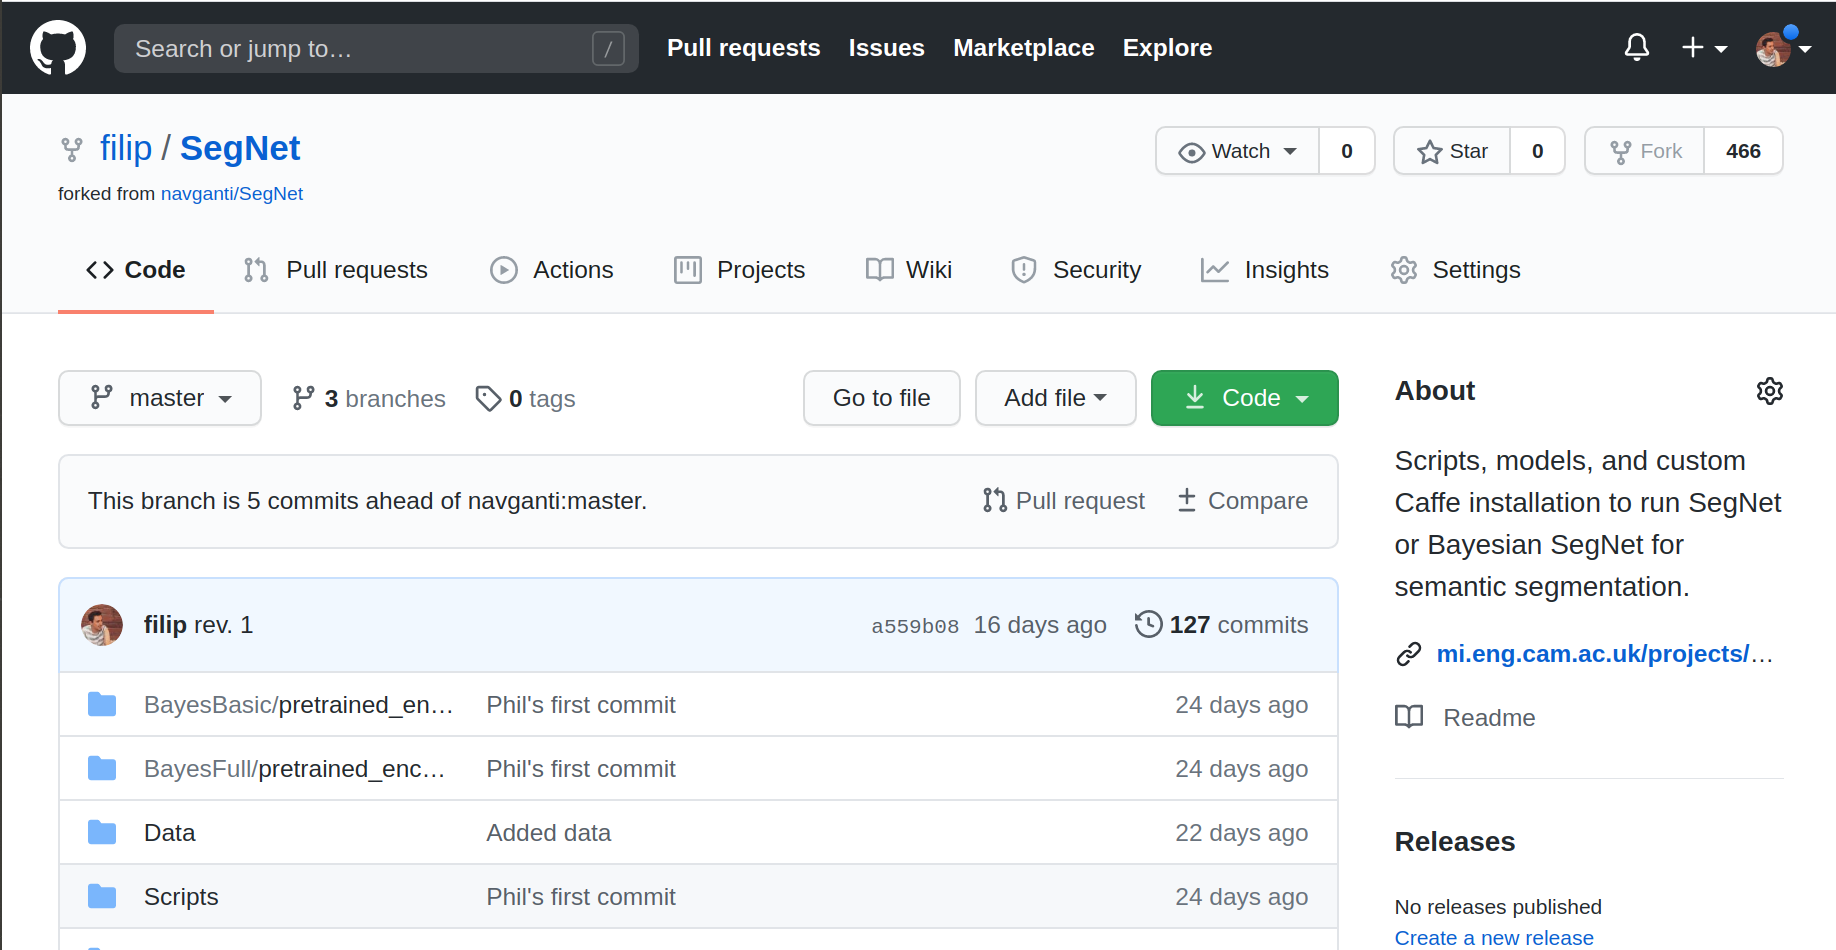
\includegraphics[width=15cm, keepaspectratio]{github.png}
	\end{center}	 	
\end{figure}
\end{frame}
% ----------------------------------------------------------------------
\begin{frame}{}
	\centering
	{\Large Děkuji za pozornost}	
\end{frame}
% ----------------------------------------------------------------------
% It is a common practice you already have reviewer(s) comments/questions before your presentation. Sometimes, it is useful to prepare extra slides to answer those questions.
\begin{frame}{Otázky oponenta}
\begin{columns}
\column{0.45\textwidth}
\begin{exampleblock}{Dotaz č. 1}
V práci je použita segmentace binární (cesta/necesta). Dala by se Vámi použitá metoda využít i pro segmentaci překážek na cestě? Pokud ano, jak velká datová množina pro trénování by musela být použita? Jak konkrétně by modifikace metody vypadala?
\end{exampleblock}

\column{0.45\textwidth}
\begin{block}{Odpověď}
SegNet je možné přenastavit na segmentaci libovolného počtu tříd. Velikost množiny: čím větší, tím lepší. Důležitý je \textbf{vyvážený výskyt všech tříd} segmentace v trénovacích datech. \\~\\

V tomto případě není nutné rozlišovat mezi ruznými druhy překážek, SegNet je všechny vyhodnotí jako 'necesta'.
\end{block}
\end{columns}
\end{frame}
% ----------------------------------------------------------------------
\begin{frame}{Trénování architektur 'enkodér-dekodér'}
\textbf{Předtrénovaná síť}
\begin{itemize}
	\item Cílem enkodéru je pouze detekovat obecné prvky v obraze
	\item Možnost použít již natrénovaný enkodér pro \textbf{inicializaci} parametrů
	\item V praxi se toto schéma používa skoro vždy!
\end{itemize}
\end{frame}
% ----------------------------------------------------------------------

\end{document}
